\documentclass[12pt]{report}
\usepackage{amsmath,amssymb,amsfonts}
\usepackage{courier}
\usepackage{graphicx}
\usepackage{hyperref}
\usepackage{listings}
\usepackage{color}
\usepackage{tikz}
\usepackage{circuitikz}
\usepackage{algorithm}
\usepackage{algpseudocode}
\usetikzlibrary{shapes,arrows, automata}
\usepackage[margin=2cm]{geometry}

\title{ECSE 426 - Microprocessor Systems\\Lab Report 2: Timers, Interrupts, Multithreaded, Interrupt-Driven Readings and Peripheral Control}
\author{Harley Wiltzer (260690006)\\Matthew Lesko (260692352)}
\date{March 19, 2018}

\definecolor{dblue}{rgb}{0.4,0.4,0.8}

\hypersetup {
	colorlinks=true,
	linkcolor=dblue
}

\tikzstyle{decision} = [diamond, draw, fill=blue!20, text badly centered, text width=2cm, node
distance=3cm]
\tikzstyle{block} = [rectangle, draw, fill=blue!20, text centered, rounded corners, minimum
height=4em, text width=3cm, node distance=5cm]
\tikzstyle{goal} = [rectangle, draw, fill=yellow!20, text centered, rounded corners, minimum
height=4em, text width=3cm, node distance=5cm]
\tikzstyle{line} = [draw, -latex']
\tikzstyle{cloud} = [draw, ellipse, fill=red!20, node distance=7cm, text centered, text width=2cm]
\tikzstyle{label} = [draw, rectangle, text centered, text width = 3cm]

\renewcommand*\thesection{\arabic{section}}

\begin{document}
\maketitle
\pagenumbering{roman}
\tableofcontents
%\let\clearpage\relax
\listoffigures
\let\clearpage\relax
\listoftables
\newpage
\pagenumbering{arabic}
\section{Abstract}
The purpose of experiment 3 is for the programmers to gain experience in utilizing timers and
interrupts to accomplish a task which involves converting an analog pulse to digital and displaying
its voltage on an LED display, effectively a voltmeter. The purpose of experiment 4 is for the
programmers to gain exposure in designing a multithreaded program on a real time operating system
(RTOS) running on an embedded system. The task of experiment 4 involves copying over experiment 3's
program and subdiving several of its features each to its own concurrently running thread, with the
goal of optimizing power usage. This report will explain in detail how the programmers implemented
the problems stated below, as well as the challenges they faced, the testing they had done, and the
conclusions they have made. By the end of the report, the reader shall understand how the timers
available on the STM32F4 board can be used to activate peripherals and generate a pulse, and
understand the implementation of multithreaded programs on embedded systems.
\section{Problem Statement}
The problem is for the developers to first implement a solution for generating a PWM pulse whose
duty cycle is controlled in order to maintain an approximately DC output voltage from a rectifier,
where the  voltage set by an input on a keypad,  Afterwards, the device
shall feed the rectifier's output to an ADC to be converted to a digital signal, and have the
signal's mean voltage be automatically displayed on an LED display. Furthermore, the program has to
be implemented with the use of concurrently-running threads running on an RTOS. The problem can be
divided into the following tasks:
\begin{itemize}
	\item Setting up a timer to act as a PWM pulse generator;
	\item Setting up a timer to activate the ADC to take an analog sample and convert it to digital;
	\item Designing a rectifier circuit component that takes the PWM pulse as input and feeds the output to the ADC;
	\item Testing and optimization of an FIR filter that reduces noise from the output signal of the ADC;
	\item Setting up the alphanumeric keypad so that the user may input their desired voltage to be displayed on an LED display;
	\item Maintaining the 7-segment display;
	\item Coding a controller function that automates the changes to be made on the PWM's duty cycle
		so that the current voltage adjusts to the target voltage set by the user;
	\item Coding a finite state machine function that enables the user to Enter and Delete digits for the target voltage, Reset the target voltage, and put the device to Sleep by using the keypad;
	\item Implementing the program's features using CMSIS-RTOS and multithreading;
	\item Reducing the power consumption of the device when it is in sleep mode using CMSIS-RTOS.
\end{itemize}
\section{Theory and Hypothesis}
Since this experiment uses components from experiment number 2, any theory for the identical components that has been mentionned in the previous lab report will be skipped. If you need to see theory for those components, and it is not mentionned here, please refer to Lab Report number 1.

\subsection{Rectifier}
A rectifier is a component that converts alternating current (AC) to direct current (DC). It does so by only allowing a one-way flow of electrons, by the use of a diode. The diode allows electric current only in the forward bias condition and blocks electric current in reverse bias condition, this allows it to act like a rectifier. The output of the diode only contains a positive half cycle, as opposed to the input having a positive and a negative half cycle [1]. The rectifier component of this experiment's device contains a diode connected in series with a parallel connection of a resistor and a capacitor.

\subsection{Multithreading and Semaphores}
The idea of multithreading is to have multiple threads execute concurrently. This allows for parallelism, more effecient use of a processor, and faster execution time. This is similar to the notion of concurrently-running processes, however, threads are not processes. One can have multiple threads running in one process, thus allowing for less overhead because the threads all share the same data [2]. Since, the threads may be sharing resources, this requires some kind of mutual exclusion to prevent threads from falling into deadlock or race-condition situations. The solution is semaphores. Semaphores allow one program to use a shared resource without having other programs use the resource at the same time. This is done by having a program wait until a semaphore is available to use before it can have access to the shared resource and execute its code. First a program waits for a semaphore, and once it is available, holds the semaphore by decrementing the semaphore's count, and executing its code. If the semaphore has a value of 0, no other program that is waiting for the same semaphore can execute. When the program using the shared resource no longer has need for the resource, it releases the semaphore by incrementing the semaphore's count, thus allowing other programs that are waiting to execute, to use the resource [2]. This resolves the problem of deadlocks and race-conditions.

\subsection{Hypothesis}
The programmers should be able to implement a solution for experiment 3 given the time allocated for
the project. The challenges one expects to face are learning how to use the keypad and implementing
a solution with it, testing of the resistor and capacitor components for the rectifier, and
implementing a solution for the different features available on the keypad with the use of a finite
state machine. Furthermore, it is expected that a simple $p$-type controller design will be
sufficient for adjusting the rectifier output voltage quickly. The programmers should be able to
implement a solution for experiment 4 given the time allocated for the project, since the majority
of the device and code is the same from experiment 3 and the students should have had experience
with multithreading and semaphores. Due to the independence of various components of the system, it
is expected for the code from experiment 3 to be easily divisible into several concurrent threads,
which would increase the efficiency of the system and readability of the code without any
non-negligible performance sacrifice.

\section{Implementation}

\subsection{PWM Pulse Generation}
The developers were tasked with designing a system that generates PWM pulses and feeds the voltage
to a rectifier circuit. Under the \hyperref[appendixtim2]{TIM3 configuration settings}, a timer, one
can see that it is configured to generate a pulse at a frequency of 500kHz, by inheriting the APB
clock of 84MHz and having a period of 168, hence having 84MHz divided by 168, yielding 500kHz. The
students have chosen to use this frequency after having tested lower frequencies, and came to the
conclusion that in order for the duty cycle to control the output voltage, the frequency had to be
elevated to at least this amount of frequency. After \hyperref[testpwm]{testing and observing}, the
students noticed that a frequency of 500kHz was suitable enough to have the duty cycle control the output voltage. The STM32F4's TIM3 hardware timer is configured to generate and output a PWM pulse channel that is assigned to a GPIO pin on the board, which can be viewed in the \hyperref[pinconfig]{GPIO pin configuration table} generated by STMCubeMX. By using a circuit wire, the programmers can feed the output of the PWM pulse channel to a circuit component on a bread board, more specifically, the rectifier.\\
The rectifier circuit holds the charge in the capacitor while a load resistance discharges the capacitor, enabling the user to influence the duty cycle to control the output voltage level. The required range for the output voltage is between 0.5V and 2.8V, hence it is required to test different configurations for the resistor and capactitor to deliver a range of output voltages that meet the requirement. The students have chosen a capacitor of 5uF and a resistor of 390 Ohms. This configuration was chosen because it achieved an output voltage range of 0.4V to roughly 2.1V. The programmers were able to observe this phenomenon after \hyperref[testpwm]{testing} multiple different configurations and came to the conclusion that the resistor and capacitor values chosen were suitable for the task.

\subsection{ADC and Timers}
Previously, the students used STM's built-in SysTick to enable the ADC. For this experiment, the
students had configured the ADC to be triggered by an STM32F4 timer, specifically TIM2. Under the
\hyperref[appendixtim2]{TIM2 configuration settings}, one can see that the timer is configured with
a prescaler of 83999 and a period of 1, which by inherting the APB clock of 84MHz, entails the timer
to a frequency of 1kHz. The reason behind this decision is so that the ADC gets activated frequently enough to take samples more often. This would allow it to be a more responsive component and allow the output voltage's RMS to be updated more accurately. One can see under the \hyperref[appendixadc]{ADC's configuration settings} that the trigger for the ADC's activation is the TIM2's trigger event.

\subsection{Filtering}
The devices uses a modified FIR filter from experiment 2 in order to reduce the noise of the ADC's signal. The two modifications are the following: 
\begin{itemize}
	\item Increasing from 5 coefficients to 10 being used in the moving average;
	\item Setting the first five coefficients to 0.05 and the last five coefficients to 0.15.
\end{itemize}
In this way, the 5 earliest samples hav have a significance of 0.05 and the 5 later samples have a significance of 0.15 when calculating the average of the 10 samples. The programmers drew this conclusion by trial and error and the empirical evidence proved that the above modifications to the FIR filter significantly reduced the signal's noise. The programmers have tested mutliple configurations, in which this report shall demonstrate three of the tested configurations. The graphs the programmers have used to determine the optimized filter can be seen in the  \hyperref[testfiltering]{Testing and Observations: Filtering}, section. After testing multile configurations, the three that are graphed in the testing section further prove that the programmers have chosen an accurate filter with coefficients: [0.15, 0.15, 0.15, 0.15, 0.15, 0.05, 0.05, 0.05, 0.05, 0.05].

%TODO These sections
\subsection{Alphanumeric Keypad}
In order to allow a user to either control the output voltage of the rectifier circuit or put the
system to sleep, it was required to integrate a keypad peripheral. The keypad has buttons arranged
in a $4\times 3$ matrix which is interpreted via the 7 pins that the keypad offers. In order to read
a given column of the keypad, one may set the keypad's corresponding column pin \texttt{HIGH} and
subsequently read all four row pins. The reading of the four row pins and the column pins are passed
through a lookup table (implemented in software) which returns the corresponding key that was
pressed (assuming only one key is pressed at any given time).\\\\
The overall strategy for processing keyboard input is as follows:
\begin{enumerate}
	\item Set the pin corresponding to the first keypad column HIGH.
	\item Poll the row pins for a short period (on the order of $100$ms).
	\item If the row pins indicate that a button was pressed, search lookup table for the
		appropriate button reading and latch it in a \texttt{reading} variable
	\item Repeat steps 2 and 3 for each of the remaining column pins.
	\item Once all column pins have been read, alert other tasks of the \texttt{reading} variable
		(via a signal in the context of an RTOS, for example) and reset \texttt{reading = -1}.
		Note that it is important to alert other tasks when no button has been pressed as well
		(indicated by \texttt{reading = -1}) in order to distinguish between a user pressing a
		button and a user holding a button.
	\item Repeat
\end{enumerate}
The above procedure assumes the keypad controller is operating concurrently with the rest of the
system, which was true in the case of Lab 4 which made use of an RTOS. However, during lab 3, this
was not at all the case. Since no signals could be sent, the finite state machine would wait for the
whole keyboard to be scanned before computing its next state. Clearly, this is rather inefficient as
the finite state machine would, first of all, have to wait approximately 300ms before each state
transition. Secondly, since most of the time the user is not pressing a button, the finite state
machine would end up polling for button presses needlessly for the majority of the CPU time. With
the threading and signal implements in FreeRTOS, this efficiency was increased greatly. In the
implementation of Lab 4, as discussed below.
%With this architecture, the keyboard may be read as follows, in algorithm 1.
%\begin{algorithm}
%	\caption{Reading the keypad}
%	\begin{algorithmic}[1]
%		\Function{ReadKeypad}{}
%			\State{$i\leftarrow 0$}
%			\While{$i < 3$}
%				\State{Wait for signal from keypad timer}\Comment{Read each column for a few ms}
%				\State{Set all column pins LOW}
%				\State{Set $i$th column pin HIGH}
%				\State{$\mathbf{x}\leftarrow$ row pin readings}
%				\State{$r\leftarrow\texttt{LUT}(\mathbf{x},i)$}
%			\EndWhile
%		\EndFunction
%	\end{algorithmic}
%\end{algorithm}

\subsection{Finite State Machine}
A finite state machine was implemented to control the functionality of the system according to the
state the system is in. The state is changed by inputs to the keypad from the user.\\\\
\begin{figure}[h]
	\begin{center}
		\caption{Finite State Machine}\label{fig1}
		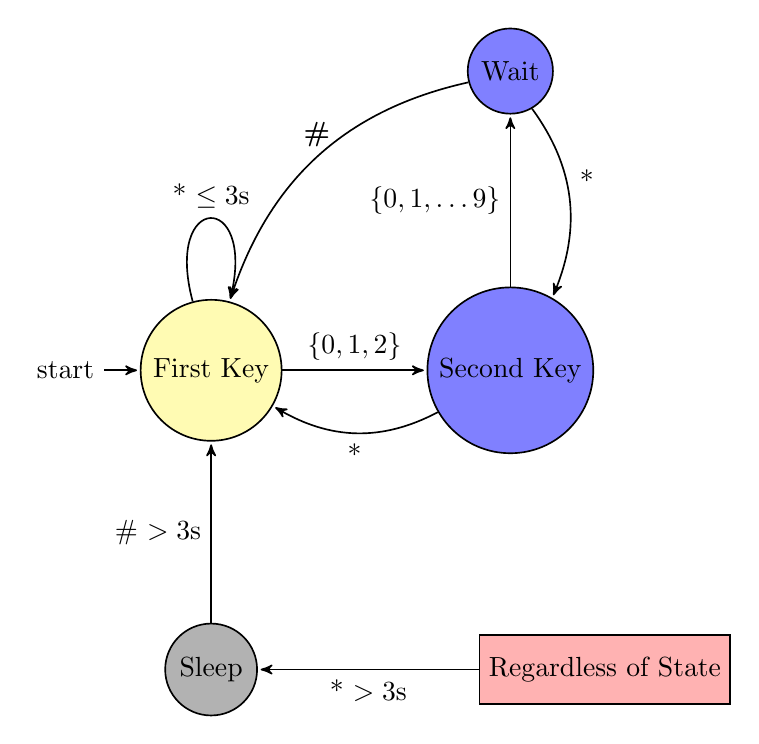
\begin{tikzpicture}[->,>=stealth',shorten >=1pt, auto, node distance=3.8cm, semithick]
			\tikzstyle{every state}=[fill=blue!50, draw]
			\node[initial, state, fill=yellow!30] (FIRST) {First Key};
			\node[state] (SECOND) [right of=FIRST] {Second Key};
			\node[state] (WAIT) [above of=SECOND] {Wait};
			\node[state, fill=gray!60] (SLEEP) [below of=FIRST] {Sleep};
			\node[state, fill=red!30, shape=rectangle, node distance=5cm] (ANY) [right of=SLEEP] {Regardless of State};
			\path (FIRST) edge node {$\{0,1,2\}$} (SECOND);
			\path (SECOND) edge node {$\{0,1,\dots 9\}$} (WAIT);
			\path (WAIT) edge [bend right] node [above] {\textbf{\#}} (FIRST);
			\path (SECOND) edge [bend left] node {*} (FIRST);
			\path (WAIT) edge [bend left] node {*} (SECOND);
			\path (FIRST) edge [loop above] node {* $\leq 3$s} (FIRST);
%			\path (FIRST) edge node {* $>3$s} (SLEEP);
%			\path (SLEEP) edge [bend left] node {\# $>3$s} (FIRST);
			\path (SLEEP) edge node {\# $>3$s} (FIRST);
			\path (ANY) edge node {* $>3$s} (SLEEP);
		\end{tikzpicture}
		\\
		\textit{Yellow states: display shows measured voltage reading}\\
		\textit{Blue states: display shows current voltage typed by user}\\
		\textit{Gray states: display is off}
	\end{center}
\end{figure}
\hyperref[fig1]{Figure 1} shows the semantics of the state transitions, which was kept exactly the same between labs
3 and 4. The arrows with labels that have inequalities are triggered when the symbol before the
inequality is held for a duration that satisfies the inequality. For example, the arrow from
``Sleep'' to ``First Key'' with the label ``\# $>3$s'' should be interpreted as ``when in the Sleep
state, if the \# key is held for more than 3 seconds, transition to the First Key state''.\\\\
Although the FSM shown shows how the states are changed, details about the output of the system are
omitted in the diagram to avoid over-cluttering it. The details about how the output of the system
changes are listed in \hyperref[table1]{Table 1}.
\begin{table}[h]
	\caption{Effect of input gestures on output}\label{table1}
	\begin{center}
		\begin{tabular}{|c|c|c|p{50mm}|}
			\hline
			Source State & Action & Destination State & Output\\\hline
			Wait & Press \# & First Key & Controller adjusts output voltage to that specified by
			the user\\\hline
			Wait & Press * & Second Key & Second input digit is erased\\\hline
			Second Key & Press * & First Key & First input digit is erased\\\hline
			\textit{Any} & Hold * for around 1s & First Key & Output voltage is set to 0V\\\hline
			\textit{Any} & Hold * for $> 3$s & Sleep & Peripherals turned off, low energy mode\\\hline
			Sleep & Hold \# for $>3$s & First Key & Periphals and threads restarted\\\hline
		\end{tabular}
	\end{center}
\end{table}
Although the state transitions were implemented identically in Labs 3 and 4, the RTOS used in Lab 4
allowed for a much more efficient FSM procedure, as was foreshadowed above. Since the FSM must wait
for a new keyboard reading before transitioning states, in Lab 3 this involved \textit{busy waiting}
before control was passed to the FSM. The SysTick timer was used to time the keyboard reading, so
the FSM would essentially wait for SysTick to count up to the value corresponding to the end of the
third column of the keypad's reading period before processing any potential state transitions. This
wastes CPU time and energy.\\\\
Using multithreading capabilities of FreeRTOS, this problem was solved in Lab 4. The keypad
processing task and FSM control task were each given their own thread, so they could run
concurrently. Furthermore, semaphores and signals were used to avoid busy waiting. Firstly, to avoid
busy waiting at the FSM, the FSM would always wait on a \textit{signal} from the keypad before
proceeding. This puts the FSM in the Waiting state, where it will not be scheduled by the kernel.
This frees up CPU time for other tasks. Whenever the keypad task process a key reading (whether that
be an actual button press, or a detection that no button is being held), the keypad task signals the
FSM task, putting its thread back in the Ready state, where it can once again be scheduled by the
kernel. Immediately after receiving the signal, the FSM sets its signal back to 0, to force itself
to wait for another signal from the keypad before the next iteration.\\\\
Although this multithreading idea does increase the efficiency of certain parts of the system, it
brings along some undesirable consequences as well. The problem of mutual exclusion is of particular
significance: if two threads run concurrently and certain data shared between the two will be
written to by the threads, the value of the data will be indeterministic and will depend on the
timing of when the threads are scheduled. Thus, we must provide a way to prevent both threads from
accessing these resources at the same time when one of them is writing to it. Additionally, this
mediation must not allow the processes to ever both wait for each other resulting in an ``infinite
loop'', called deadlock. A common solution to this problem is the use of semaphores. Semaphores
normally contain an integer $i$ that counts how many free units of the resources that it controls
are available and a queue $q$ that stores all threads that are waiting on resources to be free. When
a thread ``waits'' on a semaphore, we have $i\leftarrow i-1$, and the proceeding behavior then depends on the
sign of $i$:
\begin{itemize}
	\item When $i\geq 0$, the thread continues as usual
	\item When $i<0$, the thread enters the Waiting state (so it can no longer be scheduled by the
		dispatcher) and is enqueued in $q$
\end{itemize}
Clearly, as in the case of the signal, this efficiently allows a thread to wait until a resource is
available. When a thread is finished with a shared resource, it ``releases'' the semaphore, which
causes $i\leftarrow i+1$. Again, the proceeding behavior depends on $i$:
\begin{itemize}
	\item When $i = 1$, $x\leftarrow\texttt{dequeue}(q)$, and put $x$ in the Ready state to allow it
		to be scheduled once again
	\item Otherwise, continue like usual
\end{itemize}
This shows how threads are given permission to access a shared resource. Since this method prevents
busy waiting like in the case of the signal, it is a fairly efficient way to ensure that only one
thread can access a shared resource at a time.\\\\
In the system of Lab 4, the FSM shared one resource with the keypad task: the keypad reading itself.
To protect this shared resource, a binary semaphore was used, as the keypad reading is one resource
and thus it is either free or not free. When one of the FSM thread or the keypad thread are
accessing the keypad reading data, the other thread is put in the Waiting state to avoid wasting CPU
time. Additionally, race conditions are avoided, and there is no corruption in the key reading data
as seen by either thread. To allow both the FSM and keypad threads to run concurrently, the FSM
latches the keypad reading and stores it in another unshared variable while it has access to the
keypad reading, to effectively allow the keypad thread to continue toying with the keypad reading
while the FSM executes its tasks. This was especially convenient given the vastly different
frequencies between the two threads.
\subsection{Voltage Controller}
The main requirement of the system in Labs 3 and 4 was to maintain a reasonably constant voltage
output, independent of the load on the circuit, and allow this constant voltage to be determined by
the user in real time. To accomplish this the duty cycle of the PWM output of the board's TIM3 PWM
timer was controlled and sent through a rectifier to provide the desired load-independent
voltage.\\\\
The TIM3 PWM timer counts up to a given period value $T$, at a counting rate determined by a given
prescaler $P$. As discussed above, $T$ and $P$ where chosen such that the period of the PWM pulse
was 500kHz. Furthermore, the TIM3 PWM timer has another parameter, $\delta$, which controls the duty
cycle of the PWM pulse. Whenever the count of the timer exceeds or falls below $\delta$, the PWM
output toggles. Therefore, the fraction of the period for which the PWM pulse is high (in other
words, the duty cycle) is determined by the ratio $\delta:T$.\\\\
When $\delta$ is large, the rectifier circuit has more time to charge its capacitor, and therefore
its output voltage increases. On the other hand, when $\delta$ is low, the rectifier spends most of
its time discharging the capacitor and decreasing the voltage across it, yielding a lower output
voltage.\\\\
In order to set $\delta$ appropriately to provide the desired rectifier output, feedback from the
ADC is used. Therefore, action is taken in the ADC's conversion callback function, which is
signaled in the interrupt triggered by an ADC conversion. To modify $\delta$, a $p$-type controller
was implemented. We have, after every ADC conversion,
\begin{equation}
	\delta\leftarrow \delta + p(t - x)
\end{equation}
Where $t$ is the target voltage, $x$ is the latest (filtered) voltage reading, and $p$ is a
proportionality constant chosen experimentally to be $0.01$. The main criteria for choosing $p$
where the convergence time of the controller and its stability. For lower values of $p$, it was
found that the controller took longer to converge to an appropriate output voltage. However, for
greater values of $p$, the controller would oscillate about the desired voltage too much, resulting
in a less constant output. The value $p=0.01$ was found to be a good balance between speed and
stability. During the testing phase, it was found that the system converged to the appropriate
voltage reading in approximately $40$ms on average.

\subsection{Multithreading and System Architecture}
\hyperref[fig2]{Figure 2} shows the overall architecture of the system, including the organization of the threads in
Lab 4.\\\\
\begin{figure}[h]
	\caption{System Architecture Block Diagram}\label{fig2}
	\begin{center}
		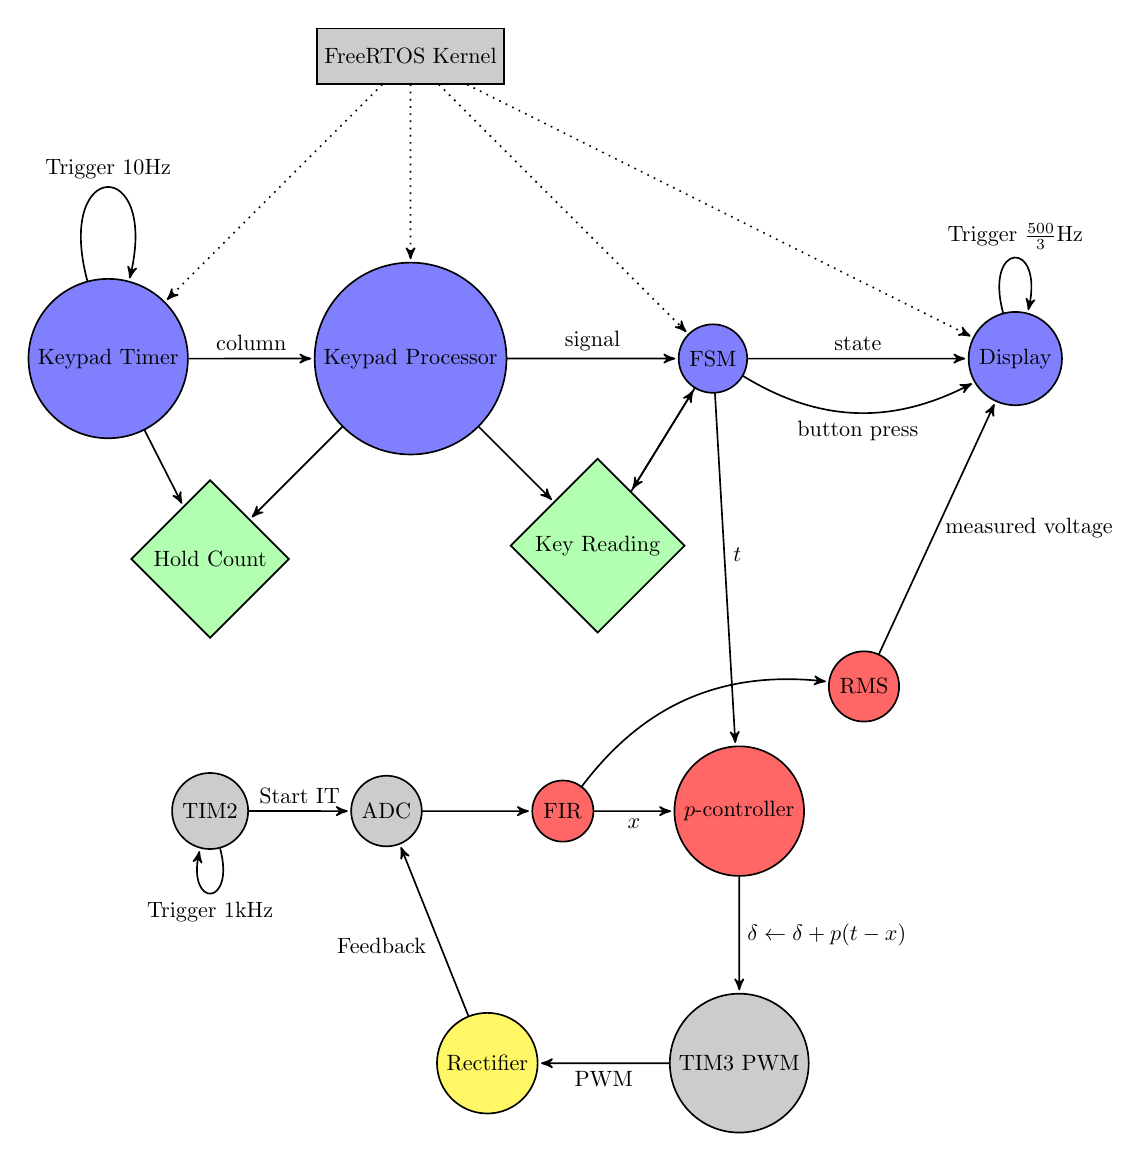
\begin{tikzpicture}[->,>=stealth',shorten >=1pt, auto, node distance=4.8cm, semithick,
			scale=0.8, transform shape]
			\tikzstyle{every state}=[fill=blue!50, draw]
			\node[state, fill=gray!40,shape=rectangle] (Kernel) {FreeRTOS Kernel};
			\node[state] (keytask) [below of=Kernel] {Keypad Processor};
			\node[state] (keytimer) [left of=keytask] {Keypad Timer};
			\node[state] (fsm) [right of=keytask] {FSM};
			\node[state] (display) [right of=fsm] {Display};
			\node[state, fill=green!30,shape=diamond, node distance=4.2cm] (reading) [below right
			of=keytask] {Key Reading};
			\node[state, fill=green!30,shape=diamond, node distance=4.5cm] (hold) [below left
			of=keytask] {Hold Count};
			\tikzstyle{every state}=[fill=red!60, draw, node distance=2.8cm]
			\node[state, fill=gray!40] (tim2) [below of=hold, node distance=4cm] {TIM2};
			\node[state, fill=gray!40] (adc) [right of=tim2] {ADC};
			\node[state] (fir) [right of=adc] {FIR};
			\node[state] (pcntrl) [right of=fir] {$p$-controller};
			\node[state] (rms) [above right of=pcntrl] {RMS};
			\node[state,fill=gray!40] (tim3) [below of=pcntrl, node distance=4cm] {TIM3 PWM};
			\node[state,fill=yellow!60] (rect) [left of=tim3, node distance=4cm] {Rectifier};

			\path (Kernel) edge[dotted] (keytimer);
			\path (Kernel) edge[dotted] (keytask);
			\path (Kernel) edge[dotted] (fsm);
			\path (Kernel) edge[dotted] (display);
			\path (keytimer) edge[loop above] node {Trigger 10Hz} (keytimer);
			\path (display) edge[loop above] node {Trigger $\frac{500}{3}$Hz} (keytimer);
			\path (keytask) edge (reading);
			\path (keytask) edge (hold);
			\path (keytask) edge node{signal} (fsm);
			\path (fsm) edge (reading);
			\path (reading) edge (fsm);
			\path (keytimer) edge (hold);
			\path (keytimer) edge node{column} (keytask);
			\path (fsm) edge node{state} (display);
			\path (fsm) edge[bend right] node[below]{button press} (display);
			\path (tim2) edge[loop below] node{Trigger 1kHz} (tim2);
			\path (tim2) edge node {Start IT} (adc);
			\path (adc) edge (fir);
			\path (fir) edge node[below]{$x$} (pcntrl);
			\path (fir) edge[bend left] (rms);
			\path (rms) edge node[right]{measured voltage} (display);
			\path (pcntrl) edge node{$\delta\leftarrow\delta +p(t-x)$} (tim3);
			\path (fsm) edge node {$t$} (pcntrl);
			\path (tim3) edge node {PWM} (rect);
			\path (rect) edge node {Feedback} (adc);
		\end{tikzpicture}
		\\
		\textit{Blue circles are threads}\\
		\textit{Green rhombi are shared resources}\\
		\textit{Red circles are software implementations}\\
		\textit{Yellow circles are electric circuits}\\
	\end{center}
\end{figure}
The design of the threads of for the FSM and keypad tasks have been discussed above. However,
certain designs of Lab 4 led to some interesting thread usage for the display and keypad timer
tasks. Firstly, powering the 7 segment display was very inefficient in Lab 3. In order to control
the timing of the refresh rates of the individual displays, display logic was included in the
SysTick interrupt callback. This is bad practice, as the SysTick callback should be as
``lightweight'' as possible to ensure the desired frequency of the interrupt. However, given the
opportunity to use threads, the display logic was implemented in its own thread entirely by OS
timers to diminish busy waiting. This once again frees up CPU time for other tasks and does not
interfere with the interrupt routine of any other time-sensitive interrupt.\\\\
Another benefit of using threads is that it makes the system more modular, which allowed more
control of which components were consuming power in the system. Therefore, an attempt was made to
decrease power usage when the device is in sleep mode. In sleep mode, the FSM and the display are
irrelevant, so their respective threads were stopped - preventing them from drawing power.
Furthermore, the peripherals such as the ADC and the timers were stopped to decrease power usage in
the dormant state. However, a more effective method would have been to deinitialize the peripherals,
which has a much greater effect on power usage.\\\\
However, with the FSM thread off in sleep mode, logic for determining when the \# key was held for 3
seconds to wake up the system had to be taken care of somewhere else, as it was initially
implemented in the FSM for Lab 3. Luckily, it was fairly simple to move this logic to the keypad
timer thread. This modification required another binary semaphore to protect a wakeup counter that
was shared between the keypad timer and the keypad processor tasks. Note that the keypad and keypad
timer threads must remain on while the device is in
sleep mode, because without them the device cannot be woken up!\\\\
Of course, the efforts made to reduce power consumption must be reversed when the device is woken
up. When the keypad timer thread detects a wakeup, it resets the state to First Key, and re-creates
the thread ID's that were defined globally. Furthermore, the peripherals such as the ADC and the
timers are started once again.


\section{Testing and Observations}

\subsection{PWM and Rectifier}\label{testpwm}

The students tested multiple configurations of resistor and capacitor values for the rectifier
circuit in order to determine which parameters allowed the largest range in DC output voltage.
Resistances in the range of $390\Omega-4.7k\Omega$ and capacitances in the range of $5\mu F-20\mu F$
were tested. These ranges were chosen since the time constants generated by those parameters satisfy
$(RC)^{-1}<<f$, where $f$ is the PWM frequency. The time constant is a measure that is related to
how long the circuit takes to charge and discharge. It was desired for this length to be far greater
than the PWM frequency so that the circuit would not have enough time to charge and discharge by
vast amounts, thereby keeping its output voltage fairly constant.\\\\

\begin{table}[h]
	\caption{Effect of rectifier parameters on its output voltage}\label{table2}
	\begin{center}
		\begin{tabular}{|c|c|c|c|}
			\hline
			Resistance (k$\Omega$) & Capacitance($\mu$F) & Duty Cycle (\%) & Output Mean Voltage (V)\\\hline
			4700 & 20 & 0.05 & 1.620\\\hline
			4700 & 20 & 0.95 & 2.150\\\hline
			4700 & 5 & 0.05 & 1.600\\\hline
			4700 & 5 & 0.95 & 2.140\\\hline
			390 & 20 & 0.05 & 0.364	\\\hline
			390 & 20 & 0.95 & 1.920\\\hline
			390 & 20 & 1.00 & 1.920\\\hline
			390 & 5 & 0.05 & 0.401	\\\hline
			390 & 5 & 0.95 & 1.930\\\hline
			390 & 5 & 1.00 & 2.105\\\hline
		\end{tabular}
	\end{center}
\end{table}
One can see from the results shown in \hyperref[table2]{Table 2} that having a small resistor (390
Ohms) and low capacitor (5uF) allow the output voltage
to yield a range roughly between 0.4V and 2.1V, making it the best suitor for the requirement of
delivering a wide range of output voltages. This configuration also has another important advantage.
Say a load resistance $\tilde{R}$ is added to the circuit. In this case, the equivalent resistance
connected across the capacitor of the rectifier circuit is
\begin{equation}
	R||\tilde{R}\equiv\frac{R\tilde{R}}{R+\tilde{R}}\leq\min(R,\tilde{R})
\end{equation}
where $R$ is the resistor used in the rectifier circuit.
Say we wish that this equivalent resistance is greater than $\alpha R$ (where $\alpha<1$), that is to say, adding the
load resistance doesn't affect the resistance of the circuit by more than some constant threshold. Then,
\begin{equation}
	\frac{R||\tilde{R}}{R} =
	\frac{\tilde{R}}{R+\tilde{R}}\geq\alpha\rightarrow\left(\frac{1-\alpha}{\alpha}\right)\tilde{R}\geq R
\end{equation}
Equation (3) shows that as $R$ grows, the smallest $\tilde{R}$ that can be loaded to the circuit
before changing the equivalent resistance by the $\alpha$ threshold grows linearly. Therefore, by
choosing a small $R$, the range of load resistances that have little effect on the equivalent
circuit is greater! This means that for a larger set of load resistances, the loading on the circuit
will have very little effect on the circuit itself, so it can be expected that the rectifier
circuit's behavior will not vary greatly by the load resistance. Therefore, a small $R$ for the
rectifier was a good choice for two main reasons: it provided a good range of output voltages, and
it is less sensitive to loading effects than a larger resistance.
\subsection{Filtering}\label{testfiltering}
One can draw comparisons from the following graphs generated by a run-time variables monitoring and
visualization tool, STM Studio[1]:\\
\begin{figure}[h] % TODO: i want my graph between the two blocks of text
	\caption{Filtered and Unfiltered Values VS Time (ms), Using Average FIR Filter}\label{fig3}
	\begin{center}
		\includegraphics[scale=0.5]{./figures/adc_5coeffs.PNG}
	\end{center}
\end{figure}
\\In \hyperref[fig3]{Figure 3}, the configuration for the filter's coefficients is [0.2, 0.2, 0.2, 0.2, 0.2].
In regular blue are the unfiltered values, and in light blue are the filtered values. This graph
demonstrates the values read at runtime of the unfilted and filtered values that passed through the
unmodified FIR filter. One can observe that there is a considerable amount of noise left from
filtering.
\begin{figure}[h] % TODO:  i want my graph between the two blocks of text
	\caption{Filtered and Unfiltered Values VS Time (ms), Using High Coeffcients for Early
	Values}\label{fig4}
	\begin{center}
		\includegraphics[scale=0.5]{./figures/adc_10coeffs_early_high_values.PNG}
	\end{center}
\end{figure}
\\In \hyperref[fig4]{Figure 4}, the configuration for the filter's coefficients is [0.05, 0.05, 0.05, 0.05,
0.05, 0.15, 0.15, 0.15, 0.15, 0.15]. This filter considers the five earliest values to each have a
significance of 0.15 and the five later values to each have a significance of 0.05. One can observe
by the graph that this filter is a considerable improvement to the unmodified version. Although, the
programmers believe that it could be optimized further.\\\\
\begin{figure}[h]% TODO:  i want my graph between the two blocks of text
	\caption{Filtered and Unfiltered Values VS Time (ms), Using High Coeffcients for Late
	Values}\label{fig5}
	\begin{center}
		\includegraphics[scale=0.5]{./figures/adc_10coeffs_late_high_values.PNG}
	\end{center}
\end{figure}
Finally, in \hyperref[fig5]{Figure 5}, the configuration for the filter's coefficients is [0.15,
	0.15, 0.15, 0.15,
0.15, 0.05, 0.05, 0.05, 0.05, 0.05]. This filter considers the five later values to each have a
significance of 0.15 and the five early values to each have a significance of 0.05. One can observe
by the graph that this filter is an improvement to the previous version. The programmers believe
that this version of the filter should perform well enough given the scope of the problem.

\section{Conclusion}
It can be concluded that the STM32 board along with a simple rectifier circuit are capable of
creating a configurable DC voltage source with considerably high resistance to loading effects. By
tuning the frequency of the PWM output of TIM3, it was possible to generate a reasonably flat output
voltage from a square wave PWM input signal. Furthermore, adjusting TIM3's \texttt{Pulse} parameter
(and thereby its duty cycle, as discussed previously) gave a sufficient range of approximately DC
output voltages from the rectifier. Interestingly enough, a \textit{very} simple control system, the
$p$-type controller, was able to automatically adjust the duty cycle extremely quickly, and the
rate at which the output voltage converged was quite good.\\\\
After implementing this system with and without a kernel and operating system, it was immediately
clear that the RTOS was very handy for improving the efficiency of the system. Certain components,
particularly the display and the keyboard, operate independently of most other components and
allowing them to run concurrently at their own frequencies was not only more CPU-efficient, but was
simpler to implement as well. Using several threads allowed a more modular design, making the code
actually easier to read and reason about in Lab 4 than Lab 3. Furthermore, Furthermore, the capacity
to prevent certain components from being scheduled by the CPU was a nice way to improve the
efficiency of the system, especially in the case of the FSM which always needs to wait for a keypad
reading before processing. Since a complete scan of the keypad is far slower than a state
transition, most of the CPU's time was wasted in the Lab 3 implementation, but using signals
eliminated this issue in Lab 4. Finally, it was possible to easily turn off threads, eliminating
their power consumption. Although the great power of threads did indeed come with great
responsibility (mutual exclusion, for example), the experience of implementing it was instructive
and overall led to a cleaner and more inuitive system design.
\newpage
\begin{appendix}\label{appendices}
	\chapter{GPIO Configuration Parameters}\label{appendixgpio}
	This appendix lists the configuration parameters set for each of the different GPIO pins (or
	classes of GPIO pins).\\\\
	\textbf{User Input Button}\\
	\begin{tabular}{|c|c|}
		\hline
		Parameter & Value\\\hline
		Mode & \texttt{GPIO\_MODE\_IT\_RISING}\\\hline
		Pull & \texttt{GPIO\_NOPULL}\\\hline
	\end{tabular}
	\newline
	\\\\
	\textbf{Display Mode LEDs (4 of these)}\\
	\begin{tabular}{|c|c|}
		\hline
		Parameter & Value\\\hline
		Mode & \texttt{GPIO\_MODE\_OUTPUT\_PP}\\\hline
		Pull & \texttt{GPIO\_NOPULL}\\\hline
		Speed & \texttt{GPIO\_SPEED\_FREQ\_LOW}\\\hline
	\end{tabular}
	\newline
	\\\\
	\textbf{Display Segment Pins (8 of these)}\\
	\begin{tabular}{|c|c|}
		\hline
		Parameter & Value\\\hline
		Mode & \texttt{GPIO\_MODE\_OUTPUT\_PP}\\\hline
		Pull & \texttt{GPIO\_NOPULL}\\\hline
		Speed & \texttt{GPIO\_SPEED\_FREQ\_LOW}\\\hline
	\end{tabular}
	\newline
	\\\\
	\textbf{Display Selector Pins (3 of these)}\\
	\begin{tabular}{|c|c|}
		\hline
		Parameter & Value\\\hline
		Mode & \texttt{GPIO\_MODE\_OUTPUT\_PP}\\\hline
		Pull & \texttt{GPIO\_NOPULL}\\\hline
		Speed & \texttt{GPIO\_SPEED\_FREQ\_LOW}\\\hline
	\end{tabular}
	\newline
	\newpage
	\chapter{ADC Configuration Settings}\label{appendixadc}
	\textbf{ADC Instance Parameters}\\
	\begin{tabular}{|c|c|}
		\hline
		Parameter & Value\\\hline
		Clock Prescaler & \texttt{ADC\_CLOCK\_SYNC\_PCLK\_DIV4}\\\hline
		Resolution & \texttt{ADC\_RESOLUTION\_8B}\\\hline
		Scan Conversion Mode & Disabled\\\hline
		Continuous Conversion Mode & Disabled\\\hline
		Discontinuous Conversion Mode & Disabled\\\hline
		External Trigger Conversion Edge & \texttt{ADC\_EXTERNALTRIGCONVEDGE\_RISING}\\\hline
		External Trigger Conversion & \texttt{ADC\_EXTERNALTRIGCONV\_T2\_TRGO}\\\hline
		Data Alignment & \texttt{ADC\_DATAALIGN\_RIGHT}\\\hline
		Number of Conversions & 1\\\hline
		DMA Continuous Requests & Disabled\\\hline
		EOC Selection & \texttt{ADC\_EOC\_SINGLE\_CONV}\\\hline
	\end{tabular}
	\newline
	\\\\
	\textbf{ADC Channel Parameters (Channel 1)}\\
	\begin{tabular}{|c|c|}
		\hline
		Parameter & Value\\\hline
		Rank & 1\\\hline
		Sampling Time & \texttt{ADC\_SAMPLETIME\_28CYCLES}\\\hline
	\end{tabular}
	\newpage
	
	\chapter{TIM2 Configuration Settings}\label{appendixtim2}
	\textbf{TIM2 Instance Parameters}\\
	\begin{tabular}{|c|c|}
		\hline
		Parameter & Value\\\hline
		Instance & \texttt{TIM2}\\\hline
		Clock Prescaler & \texttt{83999}\\\hline
		Counter Mode & \texttt{TIM\_COUNTERMODE\_UP}\\\hline
		Period & 1\\\hline
		Clock Division & \texttt{TIM\_CLOCKDIVISION\_DIV1}\\\hline
	\end{tabular}
	\newline
	\\\\
	\textbf{TIM2 Clock Source Parameters}\\
	\begin{tabular}{|c|c|}
		\hline
		Parameter & Value\\\hline
		Clock Source & \texttt{TIM\_CLOCKSOURCE\_INTERNAL}\\\hline
	\end{tabular}
	\newline
	\\\\
	\textbf{TIM2 Master Configuration Parameters}\\
	\begin{tabular}{|c|c|}
		\hline
		Parameter & Value\\\hline
		Master Output Trigger & \texttt{TIM\_TRGO\_UPDATE}\\\hline
		Master Slave Mode & \texttt{TIM\_MASTERSLAVEMODE\_DISABLE}\\\hline
	\end{tabular}
	\newpage
	
	\chapter{TIM3 Configuration Settings}\label{appendixtim3}
	\textbf{TIM3 Instance Parameters}\\
	\begin{tabular}{|c|c|}
		\hline
		Parameter & Value\\\hline
		Instance & \texttt{TIM3}\\\hline
		Clock Prescaler & \texttt{0}\\\hline
		Counter Mode & \texttt{TIM\_COUNTERMODE\_UP}\\\hline
		Period & \texttt{PWM\_PERIOD}\\\hline
		Clock Division & \texttt{TIM\_CLOCKDIVISION\_DIV1}\\\hline
	\end{tabular}
	\newline
	\\\\
	\textbf{TIM3 Master Configuration Parameters}\\
	\begin{tabular}{|c|c|}
		\hline
		Parameter & Value\\\hline
		Master Output Trigger & \texttt{TIM\_TRGO\_RESET}\\\hline
		Master Slave Mode & \texttt{TIM\_MASTERSLAVEMODE\_DISABLE}\\\hline
	\end{tabular}
	\newline
	\\\\
	\textbf{TIM3 Output Channel Parameters}\\
	\begin{tabular}{|c|c|}
		\hline
		Parameter & Value\\\hline
		OC Mode & \texttt{TIM\_OCMODE\_PWM1}\\\hline
		Pulse & \texttt{duty\_cycle * PWM\_PERIOD}\\\hline
		OC Polarity & \texttt{TIM\_OCPOLARITY\_HIGH}\\\hline
		OC Fast Mode & \texttt{TIM\_OCFAST\_DISABLE}\\\hline
	\end{tabular}	
	\newpage
	
	% TODO Add Auto Generated Code
	\chapter{HAL Cube MX Autogenerated Code}\label{mammoth}
	\begin{lstlisting}[basicstyle=\scriptsize\ttfamily]
GPIO_InitTypeDef GPIO_InitStruct;

/* GPIO Ports Clock Enable */
__HAL_RCC_GPIOE_CLK_ENABLE();
__HAL_RCC_GPIOC_CLK_ENABLE();
__HAL_RCC_GPIOH_CLK_ENABLE();
__HAL_RCC_GPIOA_CLK_ENABLE();
__HAL_RCC_GPIOB_CLK_ENABLE();
__HAL_RCC_GPIOD_CLK_ENABLE();

/*Configure GPIO pin Output Level */
HAL_GPIO_WritePin(CS_I2C_SPI_GPIO_Port, CS_I2C_SPI_Pin, GPIO_PIN_RESET);

/*Configure GPIO pin Output Level */
HAL_GPIO_WritePin(OTG_FS_PowerSwitchOn_GPIO_Port, OTG_FS_PowerSwitchOn_Pin, GPIO_PIN_SET);

/*Configure GPIO pin Output Level */
HAL_GPIO_WritePin(GPIOD, LD4_Pin | LD3_Pin | LD5_Pin | LD6_Pin | Audio_RST_Pin, GPIO_PIN_RESET);

/*Configure GPIO pin : CS_I2C_SPI_Pin */
GPIO_InitStruct.Pin = CS_I2C_SPI_Pin;
GPIO_InitStruct.Mode = GPIO_MODE_OUTPUT_PP;
GPIO_InitStruct.Pull = GPIO_NOPULL;
GPIO_InitStruct.Speed = GPIO_SPEED_FREQ_LOW;
HAL_GPIO_Init(CS_I2C_SPI_GPIO_Port, &GPIO_InitStruct);

/*Configure GPIO pin : OTG_FS_PowerSwitchOn_Pin */
GPIO_InitStruct.Pin = OTG_FS_PowerSwitchOn_Pin;
GPIO_InitStruct.Mode = GPIO_MODE_OUTPUT_PP;
GPIO_InitStruct.Pull = GPIO_NOPULL;
GPIO_InitStruct.Speed = GPIO_SPEED_FREQ_LOW;
HAL_GPIO_Init(OTG_FS_PowerSwitchOn_GPIO_Port, &GPIO_InitStruct);

/*Configure GPIO pin : PDM_OUT_Pin */
GPIO_InitStruct.Pin = PDM_OUT_Pin;
GPIO_InitStruct.Mode = GPIO_MODE_AF_PP;
GPIO_InitStruct.Pull = GPIO_NOPULL;
GPIO_InitStruct.Speed = GPIO_SPEED_FREQ_LOW;
GPIO_InitStruct.Alternate = GPIO_AF5_SPI2;
HAL_GPIO_Init(PDM_OUT_GPIO_Port, &GPIO_InitStruct);

/*Configure GPIO pin : B1_Pin */
GPIO_InitStruct.Pin = B1_Pin;
GPIO_InitStruct.Mode = GPIO_MODE_IT_RISING;
GPIO_InitStruct.Pull = GPIO_NOPULL;
HAL_GPIO_Init(B1_GPIO_Port, &GPIO_InitStruct);

/*Configure GPIO pin : I2S3_WS_Pin */
GPIO_InitStruct.Pin = I2S3_WS_Pin;
GPIO_InitStruct.Mode = GPIO_MODE_AF_PP;
GPIO_InitStruct.Pull = GPIO_NOPULL;
GPIO_InitStruct.Speed = GPIO_SPEED_FREQ_LOW;
GPIO_InitStruct.Alternate = GPIO_AF6_SPI3;
HAL_GPIO_Init(I2S3_WS_GPIO_Port, &GPIO_InitStruct);

/*Configure GPIO pins : SPI1_SCK_Pin SPI1_MISO_Pin SPI1_MOSI_Pin */
GPIO_InitStruct.Pin = SPI1_SCK_Pin | SPI1_MISO_Pin | SPI1_MOSI_Pin;
GPIO_InitStruct.Mode = GPIO_MODE_AF_PP;
GPIO_InitStruct.Pull = GPIO_NOPULL;
GPIO_InitStruct.Speed = GPIO_SPEED_FREQ_LOW;
GPIO_InitStruct.Alternate = GPIO_AF5_SPI1;
HAL_GPIO_Init(GPIOA, &GPIO_InitStruct);

/*Configure GPIO pin : BOOT1_Pin */
GPIO_InitStruct.Pin = BOOT1_Pin;
GPIO_InitStruct.Mode = GPIO_MODE_INPUT;
GPIO_InitStruct.Pull = GPIO_NOPULL;
HAL_GPIO_Init(BOOT1_GPIO_Port, &GPIO_InitStruct);

/*Configure GPIO pin : CLK_IN_Pin */
GPIO_InitStruct.Pin = CLK_IN_Pin;
GPIO_InitStruct.Mode = GPIO_MODE_AF_PP;
GPIO_InitStruct.Pull = GPIO_NOPULL;
GPIO_InitStruct.Speed = GPIO_SPEED_FREQ_LOW;
GPIO_InitStruct.Alternate = GPIO_AF5_SPI2;
HAL_GPIO_Init(CLK_IN_GPIO_Port, &GPIO_InitStruct);

/*Configure GPIO pins : LD4_Pin LD3_Pin LD5_Pin LD6_Pin 
  Audio_RST_Pin */
GPIO_InitStruct.Pin = LD4_Pin | LD3_Pin | LD5_Pin | LD6_Pin | Audio_RST_Pin;
GPIO_InitStruct.Mode = GPIO_MODE_OUTPUT_PP;
GPIO_InitStruct.Pull = GPIO_NOPULL;
GPIO_InitStruct.Speed = GPIO_SPEED_FREQ_LOW;
HAL_GPIO_Init(GPIOD, &GPIO_InitStruct);

/*Configure GPIO pins : I2S3_MCK_Pin I2S3_SCK_Pin I2S3_SD_Pin */
GPIO_InitStruct.Pin = I2S3_MCK_Pin | I2S3_SCK_Pin | I2S3_SD_Pin;
GPIO_InitStruct.Mode = GPIO_MODE_AF_PP;
GPIO_InitStruct.Pull = GPIO_NOPULL;
GPIO_InitStruct.Speed = GPIO_SPEED_FREQ_LOW;
GPIO_InitStruct.Alternate = GPIO_AF6_SPI3;
HAL_GPIO_Init(GPIOC, &GPIO_InitStruct);

/*Configure GPIO pin : VBUS_FS_Pin */
GPIO_InitStruct.Pin = VBUS_FS_Pin;
GPIO_InitStruct.Mode = GPIO_MODE_INPUT;
GPIO_InitStruct.Pull = GPIO_NOPULL;
HAL_GPIO_Init(VBUS_FS_GPIO_Port, &GPIO_InitStruct);

/*Configure GPIO pins : OTG_FS_ID_Pin OTG_FS_DM_Pin OTG_FS_DP_Pin */
GPIO_InitStruct.Pin = OTG_FS_ID_Pin | OTG_FS_DM_Pin | OTG_FS_DP_Pin;
GPIO_InitStruct.Mode = GPIO_MODE_AF_PP;
GPIO_InitStruct.Pull = GPIO_NOPULL;
GPIO_InitStruct.Speed = GPIO_SPEED_FREQ_LOW;
GPIO_InitStruct.Alternate = GPIO_AF10_OTG_FS;
HAL_GPIO_Init(GPIOA, &GPIO_InitStruct);

/*Configure GPIO pin : OTG_FS_OverCurrent_Pin */
GPIO_InitStruct.Pin = OTG_FS_OverCurrent_Pin;
GPIO_InitStruct.Mode = GPIO_MODE_INPUT;
GPIO_InitStruct.Pull = GPIO_NOPULL;
HAL_GPIO_Init(OTG_FS_OverCurrent_GPIO_Port, &GPIO_InitStruct);

/*Configure GPIO pins : Audio_SCL_Pin Audio_SDA_Pin */
GPIO_InitStruct.Pin = Audio_SCL_Pin | Audio_SDA_Pin;
GPIO_InitStruct.Mode = GPIO_MODE_AF_OD;
GPIO_InitStruct.Pull = GPIO_PULLUP;
GPIO_InitStruct.Speed = GPIO_SPEED_FREQ_LOW;
GPIO_InitStruct.Alternate = GPIO_AF4_I2C1;
HAL_GPIO_Init(GPIOB, &GPIO_InitStruct);

/*Configure GPIO pin : MEMS_INT2_Pin */
GPIO_InitStruct.Pin = MEMS_INT2_Pin;
GPIO_InitStruct.Mode = GPIO_MODE_EVT_RISING;
GPIO_InitStruct.Pull = GPIO_NOPULL;
HAL_GPIO_Init(MEMS_INT2_GPIO_Port, &GPIO_InitStruct);

/*Configure 7 segment pins*/
GPIO_InitStruct.Pin = GPIO_PIN_7 | GPIO_PIN_11 | GPIO_PIN_10 | GPIO_PIN_14 | GPIO_PIN_15;
GPIO_InitStruct.Mode = GPIO_MODE_OUTPUT_PP;
GPIO_InitStruct.Pull = GPIO_NOPULL;
GPIO_InitStruct.Speed = GPIO_SPEED_FREQ_LOW;
HAL_GPIO_Init(GPIOE, &GPIO_InitStruct);
GPIO_InitStruct.Pin = GPIO_PIN_12 | GPIO_PIN_13;
GPIO_InitStruct.Mode = GPIO_MODE_OUTPUT_PP;
GPIO_InitStruct.Pull = GPIO_NOPULL;
GPIO_InitStruct.Speed = GPIO_SPEED_FREQ_LOW;
HAL_GPIO_Init(GPIOB, &GPIO_InitStruct);
GPIO_InitStruct.Pin = GPIO_PIN_8;
GPIO_InitStruct.Mode = GPIO_MODE_OUTPUT_PP;
GPIO_InitStruct.Pull = GPIO_NOPULL;
GPIO_InitStruct.Speed = GPIO_SPEED_FREQ_LOW;
HAL_GPIO_Init(GPIOD, &GPIO_InitStruct);

/*Configure digit selector pins*/
GPIO_InitStruct.Pin = GPIO_PIN_2 | GPIO_PIN_3 | GPIO_PIN_0;
GPIO_InitStruct.Mode = GPIO_MODE_OUTPUT_PP;
GPIO_InitStruct.Pull = GPIO_NOPULL;
GPIO_InitStruct.Speed = GPIO_SPEED_FREQ_LOW;
HAL_GPIO_Init(GPIOD, &GPIO_InitStruct);

/*Configure keypad column pins*/
GPIO_InitStruct.Pin = GPIO_PIN_5 | GPIO_PIN_3 | GPIO_PIN_1;
GPIO_InitStruct.Mode = GPIO_MODE_OUTPUT_PP;
GPIO_InitStruct.Pull = GPIO_NOPULL;
GPIO_InitStruct.Speed = GPIO_SPEED_FREQ_LOW;
HAL_GPIO_Init(GPIOE, &GPIO_InitStruct);

/*Configure keypad row pins*/
GPIO_InitStruct.Pin = GPIO_PIN_8 | GPIO_PIN_7 | GPIO_PIN_5;
GPIO_InitStruct.Mode = GPIO_MODE_INPUT;
GPIO_InitStruct.Pull = GPIO_PULLDOWN;
HAL_GPIO_Init(GPIOB, &GPIO_InitStruct);
GPIO_InitStruct.Pin = GPIO_PIN_7;
GPIO_InitStruct.Mode = GPIO_MODE_INPUT;
GPIO_InitStruct.Pull = GPIO_PULLDOWN;
HAL_GPIO_Init(GPIOD, &GPIO_InitStruct);
	\end{lstlisting}
	
	\newpage
	
	\chapter{HAL GPIO Pin Configuration}\label{pinconfig}
	\begin{figure}[h]
	\label{HAL GPIO Pin Configuration}
		\begin{center}
			\includegraphics[scale=0.7]{./figures/pin_config.PNG}
			\caption{HAL's Visualization of the STM32F4's Pins Configuration}
		\end{center}
	\end{figure}
	\newpage
	
	
	\chapter{Theory References}
	\begin{itemize}
		\item 1. Tool, B. and Library, C. (2018). Rectifier Circuits | Diodes and Rectifiers | Electronics Textbook. [online] Allaboutcircuits.com. Available at: https://www.allaboutcircuits.com/textbook/semiconductors/chpt-3/rectifier-circuits/ [Accessed 18 Mar. 2018].
		\item 2. Justsoftwaresolutions.co.uk. (2018). Locks, Mutexes, and Semaphores: Types of Synchronization Objects | Just Software Solutions - Custom Software Development. [online] Available at: https://www.justsoftwaresolutions.co.uk/threading/locks-mutexes-semaphores.html [Accessed 18 Mar. 2018].
	\end{itemize}
\end{appendix}
\end{document}
